\documentclass[10pt, compress]{beamer}

\usetheme{metropolis}
\usepackage{appendixnumberbeamer}

\usepackage{tikz-dependency}
\usepackage{caption}
\usepackage{booktabs}
\usepackage{tabularx}
\usepackage{alltt}
\usepackage[scale=2]{ccicons}

\usepackage{pgfplots}
\usepgfplotslibrary{dateplot}

\usepackage{xspace}
\newcommand{\themename}{\textbf{\textsc{metropolis}}\xspace}

% commands from the paper
\newfontfamily\gtfont[Scale=1.1,Letters=SmallCaps]{Linux Libertine O}
\newcommand{\udtag}[1]{{\ll \textsc{#1}}}
\newcommand{\gtlabel}[1]{{\gtfont #1}}
\newcommand{\udlabel}[1]{{\tt #1}}
\newfontfamily\udfont[Scale=0.9,Letters=SmallCaps]{Linux Libertine O}
\newcommand{\utag}[1]{{\udfont#1}}
\newcommand{\ufeat}[1]{{\udfont#1}}
\newcommand{\tgl}[1]{{\em #1}}
\setmonofont[Scale=MatchLowercase]{DejaVu Sans Mono}
\setmainfont[Scale=MatchLowercase]{DejaVu Sans}

% commands from the paper


\newcommand{\myarrow}[1][-45]{%
  \mathrel{%
    \text{$
     \begin{tikzpicture}[baseline = -0.5ex]
       \node[inner sep=0pt,outer sep=0pt,rotate = #1] (a) at (0,0)  {$\xrightarrow{}$};
    \end{tikzpicture}
    $}%
  }%
}%




\title{Class 04: SemEval shared tasks}

\begin{document}

\maketitle


\begin{frame}{Introduction}
% SemEval (Semantic Evaluation) is an ongoing series of evaluations of computational semantic analysis systems; it evolved from the Senseval word sense evaluation series. The evaluations are intended to explore the nature of meaning in language. While meaning is intuitive to humans, transferring those intuitions to computational analysis has proved elusive.

What is SemEval ?
\begin{itemize}
  \item International competition for semantic analysis systems
  \item 20-years old
  \item Started because evaluating semantics was hard and systems
     weren't really comparable
\end{itemize}


\end{frame}

%% History and context

\begin{frame}{History}
11 instances so far:\\
\flushright
\begin{tabular}{lrlr}
           &   \textbf{Year}            & \textbf{Location} & \textbf{Tasks} \\
\hline
Senseval-1  & 	1998    & Sussex  & -- \\
Senseval-2  & 	2001    & Toulouse  & -- \\
Senseval-3  & 	2004    & Barcelona  & -- \\
\hline
SemEval-2007  & 	2007    & Prague & 19  \\
SemEval-2010  & 	2010    & Uppsala & 18  \\
SemEval-2012  & 	2012    & Montreal & 8  \\
SemEval-2013  & 	2013    & Atlanta & 14 \\
SemEval-2014  & 	2014    & Dublin & 10 \\
SemEval-2015  & 	2015    & Denver  & 18 \\
SemEval-2016  & 	2016    & San Diego & 14  \\
SemEval-2017  & 	2017    & Vancouver  & 12 \\
SemEval-2018  & 	2018    & TBA  & 12 \\
\hline
\end{tabular}

\end{frame}


%% This year 

\section{This year}

\begin{frame}{This year}

\begin{itemize}
  \item Twelve tasks in five main areas
  \begin{itemize}
     \item  Affect and creative language in tweets
     \item  Coreference
     \item  Information extraction
     \item  Lexical semantics
     \item  Reading comprehension and reasoning
  \end{itemize}
  \item SemEval-2018 will be the 12th workshop on semantic evaluation and will be located at [TBD]. 
  \item Languages represented:
  \begin{itemize} 
    \item English (12), Spanish (3), Italian (1), Arabic (1)
  \end{itemize}
\end{itemize}
%
%eng	xxxxxxxxxxxx
%spa	xxx
%ita	x
%ara	x

\end{frame}

\begin{frame}{Timeline}

\begin{tabular}{ll}

25 September & Data ready, evaluation script and baseline system available. \\
08 January   & Evaluation period starts \\
29 January   & Evaluation period ends \\
26 February  & System description paper deadline \\
2  April     & Paper notifications \\
16 April     & Camera-ready submissions due \\
\end{tabular}

Approximately 13 weeks to get a system up and running.

\end{frame}

\begin{frame}{Vyshka participation}

Why participate in a shared task ? 

\begin{itemize}
  \item Great learning experience
  \item All participants get to send a system description paper 
  \begin{itemize}
    \item Co-located with a high-level conference (NAACL, ACL, COLING, \ldots)
  \end{itemize}
  \item Looks good on CV --- both ``participated'' and ``was best in $x$''
  \begin{itemize}
    \item Especially if you're planning on applying for PhD positions
  \end{itemize}
\end{itemize}

What next ? 
\begin{itemize}
  \item Describe (most of) this year's tasks 
  \item See if any of them look interesting
  \item Check out some of the baseline systems 
\end{itemize}

\end{frame}

\section{Affect and creative language in tweets}
%%
%%    Task 1: Affect in Tweets
%%    Task 2: Multilingual Emoji Prediction
%%    Task 3: Irony Detection in English Tweets
%%

\begin{frame}{Task 1: Affect in Tweets}
% http://www.saifmohammad.com/WebDocs/AIT-2018/AIT.pdf
% Background and Significance: Existing emotion and sentiment datasets are mainly annotated categorically without an indication of degree of emotion. Further, the tasks are almost always framed as classification tasks (identify 1 among n affect categories for this sentence). In contrast, it is often useful for applications to know the degree to which an affect category is expressed in text. In this task systems have to automatically determine the intensity of affect in tweets.

Previous datasets / tasks have focussed on simple binary classification of emotion.
This task looks at how much of each emotion is felt.

For example, given a tweet:
\begin{itemize}
  \item detect the emotional intensity of \{anger, fear, joy, sadness\} from $0..1$
\end{itemize}

\begin{columns}
    \begin{column}{0.75\textwidth}
        \framebox[1.0\width]{
        
\includegraphics[width=0.9\textwidth]{graphics/twitter-post-bees.png}
        }
    \end{column}
    \begin{column}{0.2\textwidth}
        \begin{tabular}{rl}
          0.9 & Joy \\
          0.0 & Fear \\ 
          0.0 & Sadness \\ 
          0.1 & Anger \\
        \end{tabular}
    \end{column}
\end{columns}
%
\textbf{Languages:} English, Arabic, Spanish

\end{frame}

\begin{frame}[fragile]
\frametitle{Data}

Tweet ID, Tweet text, emotion, intensity

{\small
\begin{verbatim}
11615   I'm much to full of resentment      anger      0.688
11570   Blood is boiling      anger      0.729
11571   why aggravate me on purpose?      anger      0.604
11572   @DonnyMurray I'm just no offended by stuff.      anger      0.479
11574   @Matt_Lat fuming ain't the word      anger      0.646
...
\end{verbatim}
}

\end{frame}

%\begin{frame}{Possible approaches}
%% http://saifmohammad.com/WebDocs/EmoInt-2017.pdf


% corpus-based sentiment analysis lexicon e.g. instead of binary, look at N KWIC samples and calculate percentages

%\end{frame}

\begin{frame}{Task 2: Multilingual emoji prediction}
%% Given the paramount importance of visual icons for providing an additional layer of meaning to social media messages, on one hand, and the indisputable role of Twitter as one of the most important social media platforms, on the other, we propose the Emoji Prediction task. We invite participants to submit systems designed to predict, given a tweet in English or Spanish, its most likely associated emoji. We will challenge systems to predict emojis among a wide and heterogeneous emoji space. As for the experimental setting, we will remove the emoji from the tweet and ask users to predict it, ignoring tweets including more than one emoji, for simplicity purposes (same settings of [1]). We will provide data for the two tasks: 

%Training and Evaluation Data. The data for the task will consist of 500k tweets in English and 100K tweets in Spanish. The tweets were retrieved with the Twitter APIs, from October 2015 to February 2017, and geolocalized in United States and Spain. The dataset includes tweets that contain one and only one emoji, of the 20 most frequent emojis. Data will be split into Training (80%), Trial (10%) and Test (10%).

% Label set. As labels we will use the 20 most frequent emojis of each language. They are different across the English and Spanish corpora. In the following we show the distribution of the emojis for each language (numbers refer to the percentage of occurrence of each emoji).

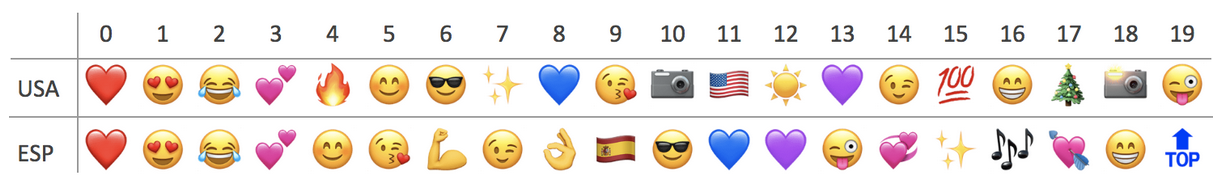
\includegraphics[width=\textwidth]{graphics/tweet-emoji-task-icons.png}

Task, given a tweet,
\begin{itemize}
  \item predict which emoji the tweet had beforehand. 
  \item single emoji per tweet.
\end{itemize}

\begin{columns}
\begin{column}{0.45\textwidth}
\centering

\includegraphics[width=\textwidth]{graphics/twitter-capdevila.png}
\end{column}
\begin{column}{0.1\textwidth}
\centering
{\Large 
$\rightarrow$
}
\end{column}
\begin{column}{0.45\textwidth}
\centering

\includegraphics[width=\textwidth]{graphics/twitter-capdevila-noemoji.png}
\end{column}
\end{columns}

\textbf{Languages}: US~English, Spanish

\end{frame}

\begin{frame}[fragile]
\frametitle{Data}

\emph{Only available after registering}

\url{https://github.com/fvancesco/Semeval2018-Task2-Emoji-Detection/}

{\small
\textbf{Training data:}
\begin{verbatim}
0    A little throwback with my favourite person @ Water Wall
2    Who never... @ A Galaxy Far Far Away
9    Birthday Kisses @ Madison, Wisconsin
\end{verbatim}
}

\textbf{Labels:}
{\small
\begin{verbatim}
0      ❤      _red_heart_      
1      😍      _smiling_face_with_hearteyes_      
2      😂      _face_with_tears_of_joy_      
...
9      😘      _face_blowing_a_kiss_      
...
\end{verbatim}
}


\end{frame}

%\begin{frame}{Possible approaches}


%\end{frame}

\begin{frame}{Task 3: Irony detection in English tweets}

\textbf{Irony}: A trope or figurative language use whose actual meaning differs from what is literally enunciated.

Two tasks:
\begin{itemize}
  \item Binary classification ironic/not ironic
  \item Four-way classification: 
  \begin{itemize}
     \item[0)] Non-ironic: {\tt \ldots And it's payday. THIS IS A GOOD FRIDAY}
     \item[1)] Polarity contrast: {\tt I love waking up with migraines \#not :'(}
     \item[2)] Situational: {\tt Event technology session is having Internet problems. \#irony}
     \item[3)] Other: {\tt @someuser Yeah keeping cricket clean, that's what he wants \#Sarcasm}
  \end{itemize}
\end{itemize}

\textbf{Languages}: English

\end{frame}

\begin{frame}[fragile]
\frametitle{Data}

\textbf{Task A:} (Binary)

{\small
\begin{verbatim}
1907    0       It's  #cute to be awake right now
2415    1       Wishing my relationship was that real 
1454    1       Good thing y days not ruined.... 
2493    0       Not this room please I don't want this
2725    0       @ajb_16 shouldn't you's be in school??
1294    0       I'm so ready to get drunk tonight
2480    1       Dead supportive family I've got. 
\end{verbatim}
}

\textbf{Task B:} (4-way)
{\small
\begin{verbatim}
1907    0       It's  #cute to be awake right now
2993    2      Spilled milk onto my boob. Oh the .
3527    2      I cant even watch anime in japan... 
3504    3      On a small diet  http://t.co/UsLZOgYmEx
2198    3      @torrentfreak We should monitor them... 
2480    1       Dead supportive family I've got. 
\end{verbatim}
}



\end{frame}

%\begin{frame}{Possible approaches}
%% https://arxiv.org/pdf/1602.03426.pdf


%\end{frame}

\section{Coreference}

\begin{frame}{Task 4: Character identification on multiparty dialogues}
%% Character Identification is an entity linking task that identifies each mention as a certain character in multiparty dialogue. Let a mention be a nominal referring to a person (e.g., she, mom, Judy), and an entity be a character in a dialogue. The goal is to assign each mention to its entity, who may or may not participate in the dialogue. For the following example, the mention "mom" is not one of the speakers; nonetheless, it clearly refers to the specific person, Judy, that could appear in some other dialogue. Identifying such mentions as real characters requires cross-document entity resolution, which makes this task challenging.

\begin{center}
  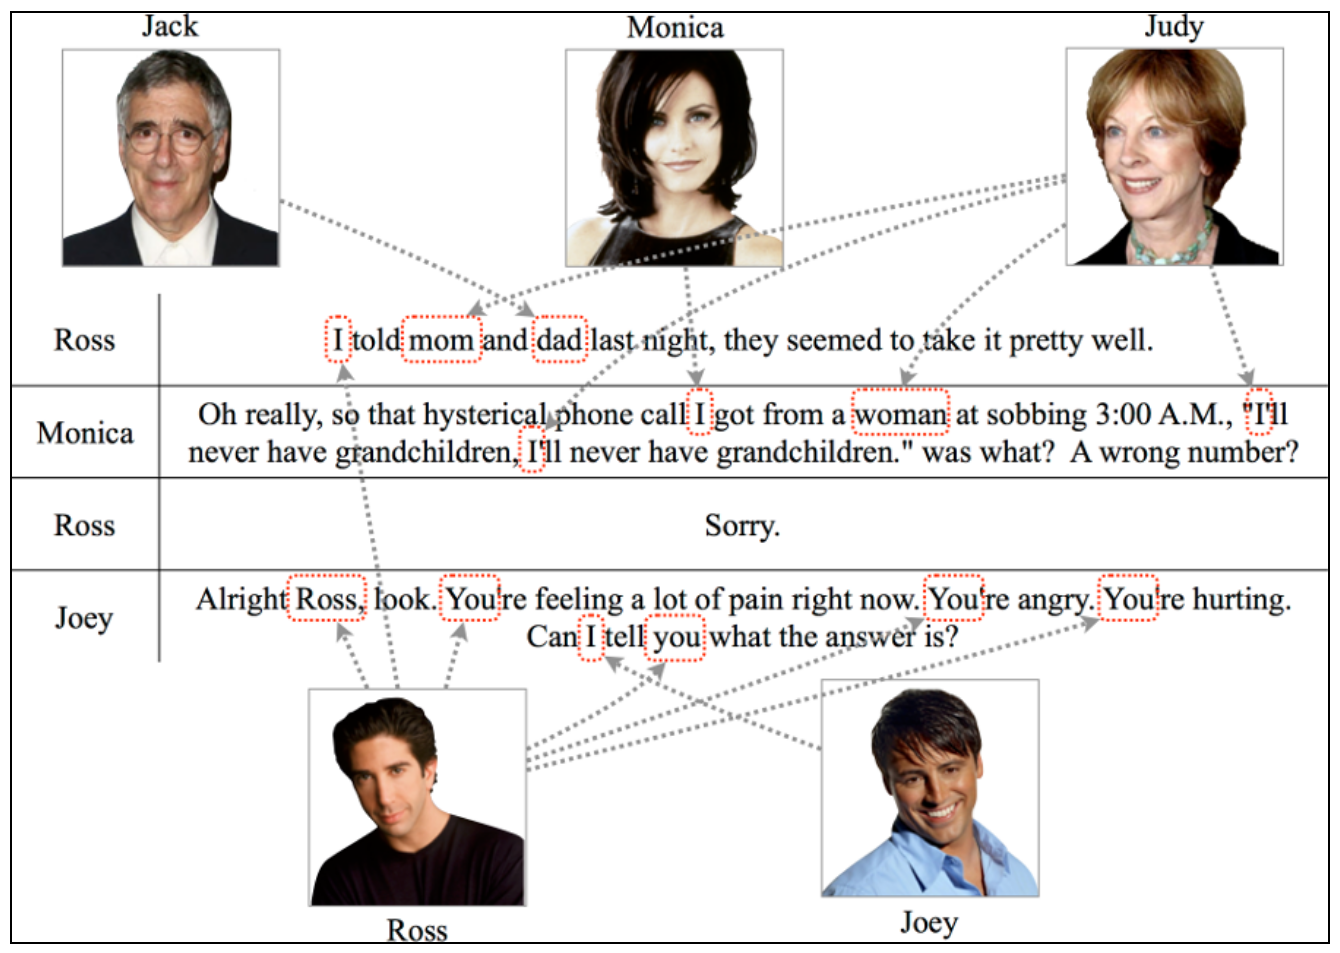
\includegraphics[width=0.6\textwidth]{graphics/coref-friends.png}
\end{center}


{\scriptsize
\begin{tabular}{lllllllllll} 
   &   &    &     &             &     &  &   & \textbf{Speaker}  &   & \textbf{Entity ID} \\
  \hline
 0 & 0 & He & PRP & (TOP(S(NP*) & he & - & - & Monica\_Geller & * & (284) \\
  0 & 1 & 's & VBZ & (VP* & be & - & - & Monica\_Geller & * & - \\
  0 & 2 & just & RB & (ADVP*) & just & - & - & Monica\_Geller & * & - \\
  0 & 3 & some & DT & (NP(NP* & some & - & - & Monica\_Geller & * & - \\
  0 & 4 & guy & NN & *) & guy & - & - & Monica\_Geller & * & (284) \\
  0 & 5 & I & PRP & (SBAR(S(NP*) & I & - & - & Monica\_Geller & * & (248) \\
  0 & 6 & work & VBP & (VP* & work & - & - & Monica\_Geller & * & - \\
  0 & 7 & with & IN & (PP*)))))) & with & - & - & Monica\_Geller & * & - \\
  0 & 8 & ! & . & *)) & ! & - & - & Monica\_Geller & * & - \\
\end{tabular}
}


\end{frame}

%\begin{frame}{Possible approaches}


%\end{frame}

\begin{frame}{Task 5: Counting events and participants in the long tail}
% The data (texts and answers) are prepared in such a way that the task deliberately exhibits large ambiguity and variation, as well as coverage of long tail phenomena by including a substantial amount of low-frequent, local events and entities.

Given a question, find news articles that correspond to the question.

\begin{center}
  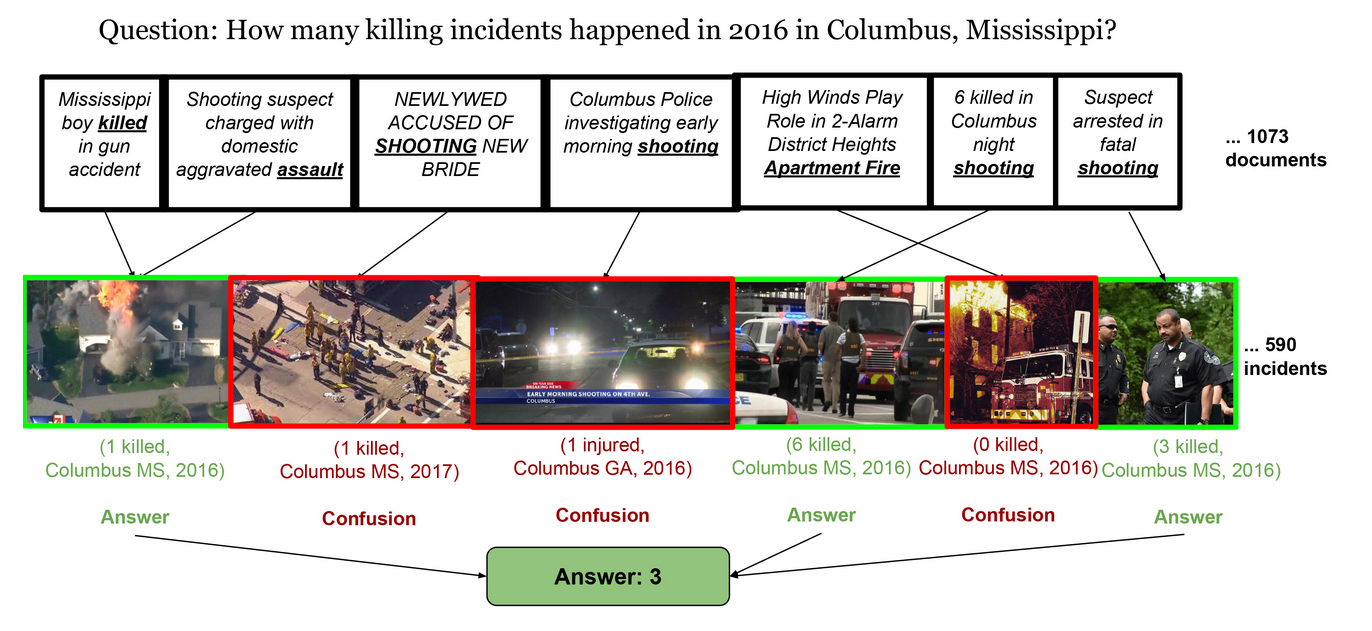
\includegraphics[width=0.8\textwidth]{graphics/events-task5-infographic.png}
\end{center}

Difficulty:
\begin{itemize}
  \item For each correct article, there are 674 incorrect articles with overlapping context 
\end{itemize}

\textbf{Languages}: English

\end{frame}

\begin{frame}
\frametitle{Data}

\emph{Only available after registering}

\end{frame}

%\begin{frame}{Possible approaches}


%\end{frame}

%% \section{Information extraction}
%% 
%% \begin{frame}{Task 6: Parsing time normalisations}
%% 
%% 
%% \end{frame}
%% 
%% %\begin{frame}{Possible approaches}
%% 
%% 
%% %\end{frame}
%% 
%% \begin{frame}{Task 7: Semantic relation extraction and classification in scientific papers}
%% 
%% 
%% \end{frame}
%% 
%% %\begin{frame}{Possible approaches}
%% 
%% 
%% %\end{frame}
%% 
%% \begin{frame}{Task 8: Semantic extraction from cybersecurity reports (SecureNLP)}
%% 
%% 
%% \end{frame}
%% 
%% %\begin{frame}{Possible approaches}
%% 
%% 
%% %\end{frame}

\section{Lexical semantics}

\begin{frame}{Task 9: Hypernym discovery}
% Hypernymy, i.e. the capability for generalization, lies at the core of human cognition. Unsurprisingly, identifying hypernymic relations has been pursued in NLP for approximately the last two decades, as successfully identifying this lexical relation contributes to improvements in Question Answering applications (Prager et al. 2008; Yahya et al. 2013) and Textual Entailment or Semantic Search systems (Hoffart et al 2014; Roller and Erk 2016). In addition, hypernymic (is-a) relations are the backbone of almost any ontology, semantic network and taxonomy (Yu et al. 2015), the latter being a useful resource for downstream tasks such as web retrieval, website navigation or records management (Bordea et al 2015).
%% Traditionally, the task of identifying hypernymic relations from text corpora has been evaluated within the broader task of Taxonomy Evaluation (e.g. SemEval-2015 task 17, SemEval-2016 task 13). Alternatively, many approaches have been specializing on Hypernym Detection, i.e. the binary task consisting of, given a pair of words, deciding whether a hypernymic relation holds between them or not. This expermental setting has already led to criticisms regarding its alleged oversimplification (Levy et al 2015; Santus et al 2016; Shwartz et al 2017; Camacho-Collados et al 2017).
%% Inspired by recent work (Espinosa-Anke et al 2016) we propose to reformulate the problem as Hypernym Discovery, i.e. given the search space of a domain’s vocabulary, and given an input concept, discover its best (set of) candidate hypernyms. In addition to making the task more realistic in terms of actual downstream applications, this novel approach also opens up complementary evaluation procedures by enabling, for instance, Information Retrieval evaluation metrics (click on the Participate/Evaluation tab for detailed information).

\begin{center}
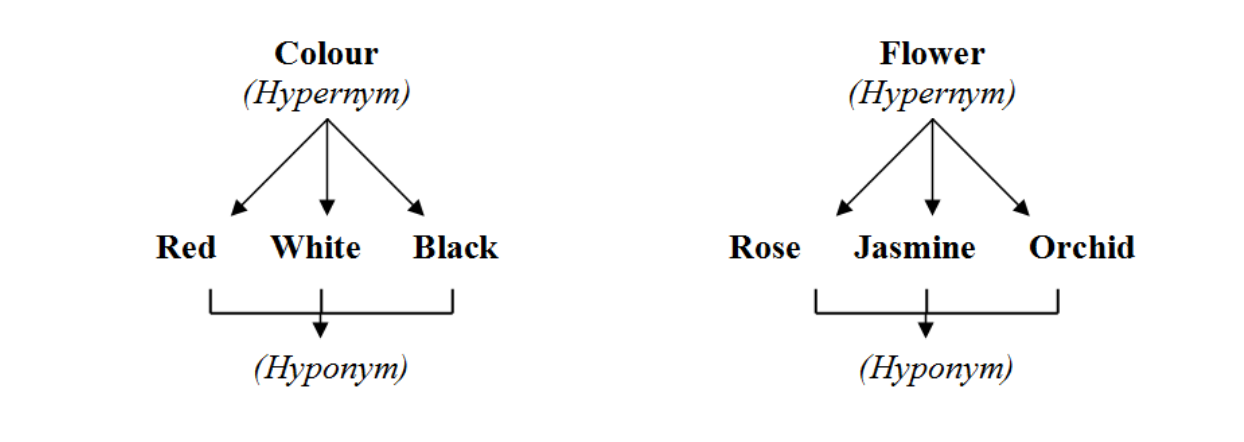
\includegraphics[width=\textwidth]{graphics/hypernymy.png}
\end{center}

\begin{center}
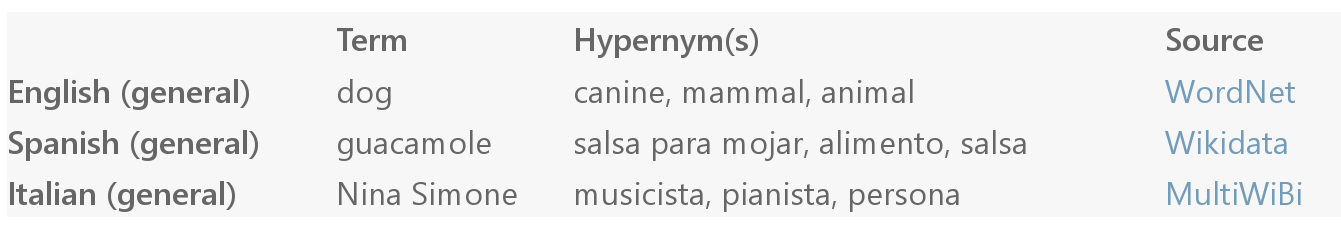
\includegraphics[width=\textwidth]{graphics/hypernyms-examples.png}
\end{center}

\textbf{Languages}: English, Spanish, Italian

\end{frame}

\begin{frame}[fragile]
\frametitle{Data}

\textbf{Input:}
{\small
\begin{verbatim}
pollution        Concept
\end{verbatim}
}

\textbf{Output:}
{\small
\begin{verbatim}
dirtiness
dirtying
environmental condition
impurity
sanitary condition
uncleanness
\end{verbatim}
}

\end{frame}

%\begin{frame}{Possible approaches}


%\end{frame}

\begin{frame}{Task 10: Capturing discriminative attributes}
%% State of art semantic models do an excellent job at detecting semantic similarity, a traditional semantic task; for example, a model will be able to tell that cappuccino, espresso and americano are similar to each other. It is obvious, however, that no model can claim to capture semantic competence if it does not, in addition to similarity, predict semantic differences between words. If you can tell that americano is similar to capuccino and espresso but you can't tell the difference between them, you don't know what americano is. As a consequence, any semantic model that is only good at similarity detection will be of limited practical use.

\begin{itemize}
  \item Current models are great at detecting similarity
  \item But do not predict semantic differences
  \item If you only know what something is like but can't tell the difference it is a problem for your model
\end{itemize}

\begin{columns}
  \begin{column}{0.3\textwidth}
    \centering
    
\includegraphics[width=\textwidth]{graphics/discrim-cappuccino.jpg}
  \end{column}
  \begin{column}{0.3\textwidth}
    \centering
    
\includegraphics[width=\textwidth]{graphics/discrim-espresso.jpg}
  \end{column}
  \begin{column}{0.3\textwidth}
    \centering
    
\includegraphics[width=\textwidth]{graphics/discrim-americano.jpg}
  \end{column}
\end{columns}

The task:
\begin{itemize}
  \item Given a triple {\tt (cappucino, americano, milk)}, return
  \begin{itemize}
  \item 1 {\tt is a semantic difference}
  \item 0 {\tt is not a semantic difference}
  \end{itemize}
\end{itemize}
%% To fill this gap, we propose a novel task of semantic difference detection. The goal of our proposed task is to predict whether a word is a discriminative attribute between two other words. For example, given the words apple and banana, is the word red a discriminative attribute?
%%Semantic difference is a ternary relation between two concepts (apple, banana) and a discriminative feature (red) that characterizes the first concept but not the other. By its nature, semantic difference detection is a binary classification task: given a triple apple,banana,red, the task is to determine whether it exemplifies a semantic difference or not.

\textbf{Languages}: English

\end{frame}

\begin{frame}
\frametitle{Data}

\emph{Only available after registering}

\end{frame}


%\begin{frame}{Possible approaches}


%\end{frame}

\section{Reading comprehension and reasoning}

\begin{frame}{Task 11: Machine comprehension using commonsense knowledge}
%% This task assesses how the inclusion of commonsense knowledge in the form of script knowledge would benefit machine comprehension systems. Script knowledge is defined as the knowledge about everyday activities, i.e. sequences of events describing stereotypical human activities (also called scenarios), for example baking a cake, taking a bus, etc. In addition to what is mentioned in the text, a substantial number of questions require inference using script knowledge about different scenarios, i.e. answering the questions requires knowledge beyond the facts mentioned in the text. 
 
\framebox{\parbox{\dimexpr\linewidth-2\fboxsep-2\fboxrule}{\itshape%
 \alert<2>{My garden was looking a little empty, so I decided} I would plant something. I went out and bought tree seeds. I found a spot that looked like it would get enough sunshine. There, I dug a hole for the seeds. Once that was done, I took my watering can and watered the seeds.
}}

~\\
~\\

\begin{columns}
  \begin{column}{0.5\textwidth}
   \alert<2>{A. Why was the tree planted?}
      \begin{itemize}
      \item    to get enough sunshine
      \item    \alert<2>{the garden looks empty}
      \item    they were forced
      \item    the soil was moist
      \end{itemize}
  \end{column}
  \begin{column}{0.5\textwidth}
   \alert<3>{B. What was used to dig the hole?}
      \begin{itemize}
      \item    the wind
      \item    a tablespoon
      \item    \alert<3>{a trowel} \textbf{[?]}
      \item    their bare hands
      \end{itemize}
  \end{column}
\end{columns}

~\\

\textbf{Languages}: English

\end{frame}

\begin{frame}
\frametitle{Data}

\emph{Only available after registering}

\end{frame}



%\begin{frame}{Possible approaches}


%\end{frame}

\begin{frame}{Task 12: Argument reasoning comprehension task}
% Reasoning is a crucial part of natural language argumentation. In order to comprehend an argument, one has to reconstruct and analyze its reasoning. As arguments are highly contextualized, most reasoning-related content is left implicit and usually presupposed. Thus, argument comprehension requires not only language understanding and logic skills, but it also heavily depends on common sense. We define a new task, argument reasoning comprehension. Given a natural language argument with a reason and a claim, the goal is to choose the correct implicit reasoning from two options. The challenging factor is that both options are plausible and lexically very close while leading to contradicting claims. We created a new freely licensed dataset based on authentic arguments from news comments.

Given an argument, with a reason and a claim, the goal is to choose the correct implicit reasoning from two options.

% warrant0|||	warrant1	correctLabelW0orW1	reason	claim	debateTitle	debateInfo
%Australians are nothing like Americans	||| Australians are like Americans|||	1|||	It works for Australia.	Voting should be mandatory|||	Should Voting Be Mandatory?|||	Or are there already too many people casting ballots?

%scholarships would give women a chance to study	scholarships would take women from the home	0	Miss America gives honors and education scholarships.	Miss America is good for women	There She Is, Miss America	In 1968, feminists gathered in Atlantic City to protest the Miss America pageant, calling it racist and sexist. Is this beauty contest bad for women?

\framebox{\parbox{\textwidth}{
\textbf{Topic:} Should voting be mandatory?

\textbf{Additional info:} Or are there already too many people casting ballots?

\textbf{Argument:} It works for Australia. And since [\ldots] voting should be mandatory.
\begin{itemize}
  \item[(a)] Australians are nothing like Americans
  \item[(b)] Australians are like Americans
\end{itemize}
}}



\textbf{Languages}: US~English

\end{frame}

\begin{frame}[fragile]
\frametitle{Data}

\url{https://github.com/habernal/semeval2018-task12}

% warrant0|||	warrant1	correctLabelW0orW1	reason	claim	debateTitle	debateInfo
%Australians are nothing like Americans	||| Australians are like Americans|||	1|||	It works for Australia.	Voting should be mandatory|||	Should Voting Be Mandatory?|||	Or are there already too many people casting ballots?

\textbf{TSV file}:

{\small
\begin{verbatim}
warrant0        Australians are nothing like Americans
warrant1        Australians are like Americans
correctLabel    1
reason          It works for Australia. 
claim           Voting should be mandatory
debateTitle     Should Voting Be Mandatory?
debateInfo      Or are there already too many people casting ballots?
\end{verbatim}
}

\end{frame}

%\begin{frame}{Possible approaches}


%\end{frame}

\section{Practical}

\begin{frame}{Practical}

\begin{center}
\url{http://alt.qcri.org/semeval2018/index.php?id=tasks}
\end{center}

\begin{itemize}
  \item Choose a task
  \item Read the description
  \item Look at the provided data
\end{itemize}

\begin{itemize}
  \item Run the baseline system (Irony detection, argument reasoning)
% Irony detection
% argument reasoning
  \item Write your own simple baseline (Everything else)
\end{itemize}

\begin{itemize}
  \item Run the evaluation script on the baseline
  \item Think of ways to improve the baseline
\end{itemize}

\end{frame}


\end{document}
